\documentclass[10pt,a4paper,oneside]{report}

\usepackage[utf8]{inputenc}
\usepackage[italian]{babel}
\usepackage{amsmath}
\usepackage{amsfonts}
\usepackage{amssymb}

\usepackage{listings}
\usepackage{rotating}
\bibliographystyle{IEEEtran}

\lstset{basicstyle=\small\ttfamily, frame=lines, breaklines=true,
emph={obj,int,bool,State,Top,Transitions,Class,is,True,False,null,Vars,Signals},
emphstyle=\bfseries
}
%\newif\ifpdf
%\ifx\pdfoutput\undefined
%\pdffalse
%\else
%\pdfoutput=1
%\pdftrue
%\fi
%\ifpdf
%\usepackage{graphicx}
%\usepackage{epstopdf}
%\DeclareGraphicsRule{.eps}{pdf}{.pdf}{`epstopdf #1}
%\pdfcompresslevel=9
%\else
%\usepackage{graphicx}
%\fi 
\author{Luca Baldesi, Luca Melis, Simone Macaluso}
\title{Modellazione di un sistema di
Interlocking Ferroviario Distribuito
tramite UML Model Checker
}

\begin{document}
\maketitle
\tableofcontents
\chapter*{Introduzione}
Lo scopo di questo elaborato è quello di modellare un sistema di
\emph{interlocking ferroviario distribuito} e di testarne le proprietà di safety e di stabilizzazione. L'automa e il model checking per tali caratteristiche saranno sviluppati tramite UML Model Checker \footnote{http://fmtlab.isti.cnr.it/umc/V3.9/umc.html}, un software per lo studio accademico di model based development. Il nostro lavoro si baserà su quello preesistente descritto in \cite{Paolieri} e in \cite{RossettoRocciolo}. In particolare introdurremo nel modello i semafori come ulteriore raffinamento al sistema di interlocking e proporremo dei casi di test e delle configurazioni della rete di maggiore complessità.

Il resto del documento è composto come segue:
Nel capitolo \ref{cap:interlocking} viene presentato il problema dell'interlocking distribuito in ambito ferroviario con la specifica di come un treno possa prenotare un itinerario nel nostro modello. Nel capitolo \ref{cap:modelling} viene descritto il modello da noi implementato e nel capitolo \ref{cap:properties} le proprietà che abbiamo verificato per il nostro modello.

Nelle appendici \ref{cap:umc} e \ref{cap:code} vengono riportate le informazioni relative al particolare strumento di model checking che abbiamo usato e il codice relativo completo del nostro modello.
\chapter{Interlocking ferroviario}
\label{cap:interlocking}
%Che cos'è l'interlocking
Tramite un sistema di \textit{interlocking ferroviario} è possibile gestire una parte di tracciato su una rete ferroviaria e quindi permettere ai treni di effettuare richieste di prenotazione dei percorsi.

A differenza di un sistema centralizzato, in cui un unico centro di elaborazione si occupa di inviare i comandi ad ogni sezione del tracciato, in un sistema di \textit{interlocking distribuito} ogni elemento della rete è in grado di eseguire in modo indipendente i propri compiti e di collaborare con i nodi adiacenti nel percorso richiesto dal treno.
\section{Elementi del tracciato}
E' possibile vedere una rete ferroviaria come un grafo $G =(V,E) $ dove i vertici $V$ sono i nodi del tracciato e gli archi $E$ sono costruiti tramite una relazione di adiacenza $R \subseteq V \times V$. in cui:
\begin{itemize}
\item un arco $e=(v,v')$ assume che $v$ sia un adiacente sinistro di $v'$
\item un arco $e=(v',v'')$ assume che $v''$ sia un adiacente destro di $v'$
\end{itemize}
Un nodo della rete può essere:
\begin{itemize}
\item \textbf{Circuito di Binario} è un tratto di binario e può avere soltanto un adiacente destro e un adiacente sinistro. Un circuito di binario può essere una stazione di fermata del treno e una stazione di fermata del treno può essere \emph{outer station} se è concettualmente adiacente con altri tracciati non rappresentati nel grafo della rete;
\item \textbf{Scambio} è un punto di diramazione o di confluenza. A seconda dell'orientazione fisica, uno scambio può essere \textit{normale} o \textit{rovescio};
\item \textbf{Segnale} o \emph{Semaforo} rappresenta un segnale adiacente a un \emph{circuito di binario} e uno \emph{Scambio}. La sua funzione è di protezione dell'unico nodo ad esso adiacente di tipo \emph{circuito di binario}.  L'introduzione di questa tipologia di nodi rompe la simmetria di percorribilità del tracciato in quanto i nodi di questa classe sono adiacenti negli itinerari solo nella direzione \emph{circuito di binario}-\textgreater\emph{Scambio}.
\end{itemize}
Su tale grafo non esistono cicli o cappi (nodi che hanno se stessi come adiacenti).
Un \emph{itinerario} sul tracciato può quindi essere visto come un percorso nel grafo della rete vincolato ad avere il primo e ultimo nodo di tipo \emph{circuito di binario}.
\section{Funzionalità del sistema di Interlocking}
Le funzioni fornite dal sistema di \emph{Interlocking} sono :
\begin{itemize}
\item prenotazioni di uno o più itinerari;
\item cancellazione di itinerari prenotati;
\item liberazione dell'itinerario dopo che il treno è transitato;
\item liberazione del tracciato all'arrivo del treno nelle stazioni terminali.
\end{itemize}

\paragraph*{Prenotazione Itinerario}
La prenotazione dell'itinerario si effettua tramite il protocollo \emph{Linear Two Phase Commit Protocol } (2PC) in cui ogni nodo della rete facente parte dell'itinerario effettua un doppio scambio di messaggi.

Ogni nodo conosce il suo successore e il suo predecessore lungo il percorso associato all'itinerario richiesto ed inoltre, il primo e l'ultimo nodo conoscono la loro posizione nel percorso.

La richiesta dell'itinerario viene effettuata dal treno tramite un messaggio di \emph{request} inoltrato direttamente al primo nodo (vincolato a essere un circuito di binario). Ogni nodo del percorso, se libero, diviene \emph{reserved} e propaga la \emph{request} al nodo successore fino all'ultimo nodo il quale invia a ritroso un messaggio di \emph{acknowledge} che, se tutti i nodi dell'itinerario sono disponibili , sarà propagato fino al primo nodo.

A seguito del messaggio di \emph{acknowledge}, il primo nodo invierà un \emph{commit} che percorrerà nuovamente il cammino e sarà riscontrato da un messaggio di \emph{agree} emesso dall'ultimo nodo.

Alla ricezione del messaggio di \emph{agree} , il primo nodo comunica al treno la disponibilità dell'itinerario permettendo quindi al treno di iniziare a muoversi e di arrivare a destinazione.

Un nodo non libero rigetta la \emph{request} con un messaggio di \emph{negative acknowledge} che provoca la liberazione del nodo che lo riceve e che si incarica, a sua volta, di propagarlo.

\paragraph*{Cancellazione Itinerario}
La fase relativa alla cancellazione di un itinerario è stata concepita come una versione a singola fase del 2PC, in quanto i nodi risultano già essere in stato \emph{reserved}.

Il treno che intende cancellare un itinerario invia un messaggio di \emph{abort}. I nodi che ricevono tale messaggio si portano nello stato di \emph{aborting} e inoltrano il messaggio al nodo successore, fino all'ultimo nodo del percorso.

L'ultimo nodo del percorso diviene libero e inoltra un messaggio di \emph{cancel} in senso inverso provocando la liberazione di tutti gli altri nodi dell'itinerario. Quando il messaggio di \emph{cancel} raggiunge il primo nodo, l'itinerario risulta essere cancellato.

\paragraph*{Liberazione Itinerario}
Una volta che il treno è transitato su un nodo della rete, quest'ultimo viene subito liberato per permettere la prenotazione di nuovi itinerari passanti per quel nodo.
\paragraph*{Liberazione tracciato}
Nel momento in cui un treno giunge nell'ultimo nodo del suo percorso (qualora esso sia \emph{outer station}), si deve poter far uscire il treno stesso dal tracciato.
In particolare, tale soluzione permette al treno di poter entrare in un altro tracciato.

Per poter fare ciò, i circuiti di binario che rappresentano \emph{outer station} possono, tramite il comando ``free'', permettere la liberazione del tracciato consentendo quindi al treno di muoversi verso l'esterno.


\chapter{Modellazione del sistema}
\label{cap:modelling}
Il modello realizzato offre le funzionalità sopra descritte implementando un
sistema di \textit{Interlocking Distribuito} di nodi di tracciati e treni.
\section{Tracciato e itinerari}
Il tracciato relativo al nostro progetto è composto da:
\begin{itemize}
  \item cinque Circuiti di Binario (GA1, GA2, GA3, GA4, GA5) di cui 
  \begin{itemize}
    \item GA1 e GA4 sono \textit{outer\_station},
    \item GA5 è associato a un binario morto;
	\end{itemize}
	\item tre locazioni di scambio (W1, W2, W3);
	\item sette semafori
	\begin{itemize}
	  \item A per le segnalazioni nella direzione GA1-\textgreater W1,
	  \item P1 per le segnalazioni nella direzione GA2-\textgreater W1,
	  \item P2 per le segnalazioni nella direzione GA3-\textgreater W1,
	  \item N2 per le segnalazioni nella direzione GA2-\textgreater W2,
	  \item N3 per le segnalazioni nella direzione GA3-\textgreater W3,
	  \item F per le segnalazioni nella direzione GA4-\textgreater W2,
	  \item S10 per controllare l'uscita dal binario morto GA5.
	 \end{itemize} 
\end{itemize}

\begin{figure}
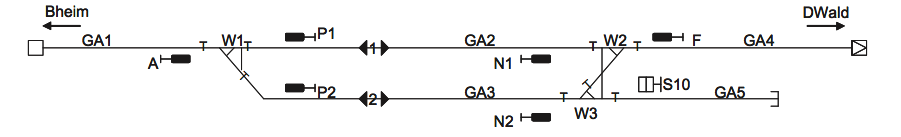
\includegraphics[width=13.5cm]{imgs/reteInterlocking.png}
\caption{Tracciato ferroviario utilizzato per la simulazione}\label{fig:X}
\end{figure}



Nel tracciato illustrato sono possibili i seguenti itinerari:
\begin{enumerate}
  \item GA1 A W1 GA2
  \item GA1 A W1 GA2 N1 W2 GA4
  \item GA1 A W1 GA3
  \item GA1 A W1 GA3 N2 W3 W2 GA4
  \item GA1 A W1 GA3 N2 W3 GA5
  \item GA4 F W2 GA2
  \item GA4 F W2 GA2 P1 W1 GA1
  \item GA4 F W2 W3 GA3
  \item GA4 F W2 W3 GA3 P2 W1 GA1
  \item GA5 S10 W3 GA3
  \item GA2 P1 W1 GA1
  \item GA2 N1 W2 GA4
  \item GA3 P2 W1 GA1
  \item GA3 N2 W3 W2 GA4
  \item GA3 N2 W3 GA5
\end{enumerate}

\section{Modello del Circuito di Binario}
Il Circuito di Binario è modellato con la classe \textit{TrackCircuit} la quale
è a conoscenza dei Circuiti di Binario precedenti e successivi (variabili
\textit{prev} e \textit{next}) per ogni possibile itinerario, sa istantaneamente
se è presente un treno (varibile \textit{train}), inoltre utilizza la variabile
booleana \textit{outer\_station} per sapere se è una stazione esterna nel
tracciato considerato. Tutte queste varibili vanno assegnate in fase di creazione di ogni
singolo oggetto.

Il comportamento dinamico del \textit{TrackCircuit} è rappresentato nella figura
\ref{fig:Circuito} dove sono evidenziati sia gli stati in cui un Circuito di Binario
può trovarsi sia quali segnali permettono le trasizioni.

\begin{sidewaysfigure}

\centering
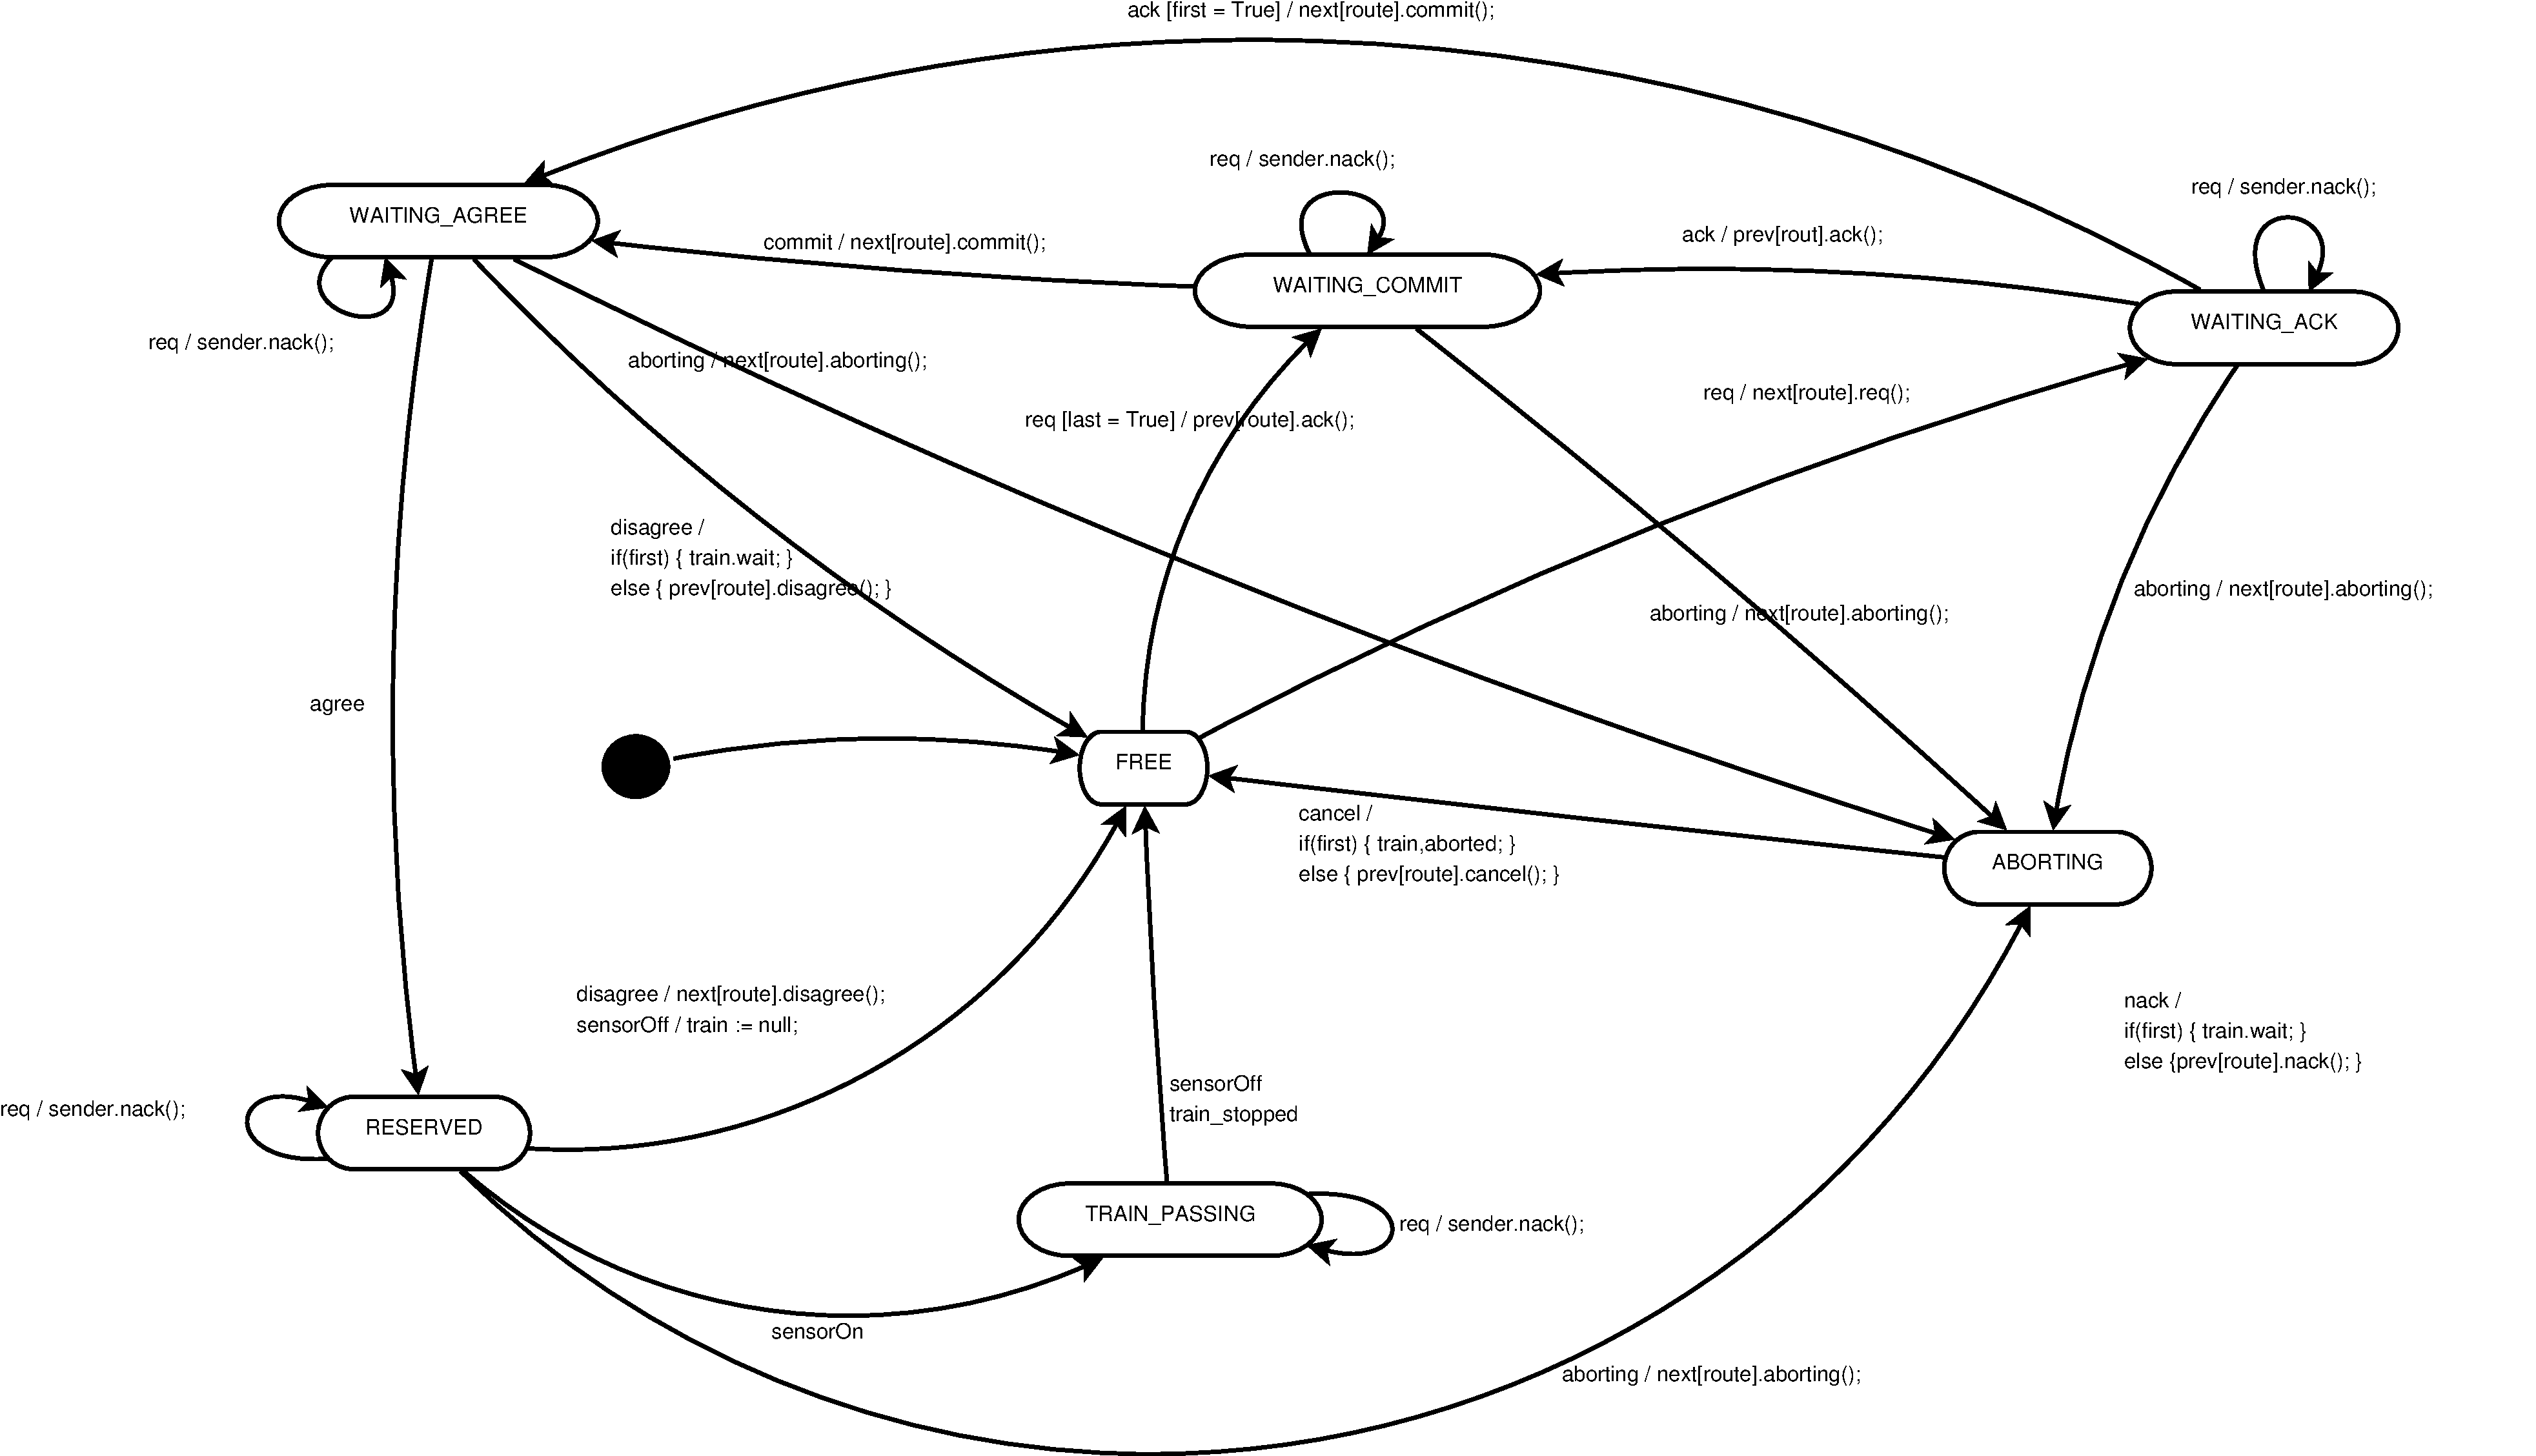
\includegraphics[width=24cm]{imgs/TrackCircuit.pdf}

\caption{Diagramma di variazione degli stati del Circuito
di Binario}\label{fig:Circuito}

\end{sidewaysfigure}



I segnali che possono essere elaborati dal \textit{TrackCircuit} sono:
\begin{itemize}
\item \textbf{Request} Il segnale \textit{req(sender, dest, route)} indica una
richiesta di prenotazione per l’itinerario route da parte dell’oggetto
\textit{sender} (un Treno, uno Scambio oppure un altro Circuito di Binario).
Quando viene ricevuto può essere rifiutato qualora lo stato corrente non sia
FREE rispondendo con un segnale \textit{nack} (o col segnale \textit{wait} se è
il primo nodo dell’itinerario), oppure può essere accettato
eseguendo la transizione nello stato \textit{WAITING\_ACK} e propagando la
richiesta al nodo successivo dell’itinerario. Se ci troviamo sul nodo finale lo
stato diverrà \textit{WAITING\_COMMIT} e non viene propagato nessun messaggio,
ma si risponde al mittente con un messaggio di \textit{ack}.

\item \textbf{Acknowledgement} Il segnale \textit{ack(sender, dest, route)} indica un
riscontro positivo alla richiesta di prenotazione relativo all’itinerario route da parte
dell’oggetto sender. Un nodo che riceve questo messaggio ha precedentemente
propagato un messaggio di req e si trova nello stato \textit{WAITING\_ACK},
quindi propaga l’ack al nodo precedente sull’itinerario e si pone in attesa del
\textit{commit} eseguendo la transizione allo stato \textit{WAITING\_COMMIT}. Se
a ricevere l’\textit{ack} è il primo nodo dell’itinerario questo si porta
direttamente nello stato \textit{WAITING\_AGREE} e spedisce un messaggio di
\textit{commit} in avanti.

\item \textbf{Negative Acknowledgement} Il segnale \textit{nack(sender, dest, route)}
rappresenta un riscontro negativo alla richiesta di prenotazione per l’itinerario route da parte
dell’oggetto sender. Un nodo che riceve questo messaggio ha precedentemente
propagato un messaggio req e poiché la prima fase del 2PC è fallita, propaga il
nack al nodo precedente sull’itinerario e ritorna allo stato FREE in attesa di una
nuova richiesta di prenotazione.

\item \textbf{Commit} Il segnale \textit{commit(sender, dest, route)} indica un
commando di “conferma prenotazione” per l’itinerario route inoltrata dall’oggetto sender. Un nodo
che riceve questo messaggio ha precedentemente propagato i messaggi req e ack
dunque si trova in \textit{WAITING\_COMMIT} e alla sua ricezione lo propaga al
nodo successivo e si pone nello stato \textit{WAITING\_AGREE}. Se il nodo è
l’ultimo dell’itinerario invece che inoltrare il \textit{commit} spedisce
indietro un messaggio \textit{agree} e si porta direttamente in
\textit{RESERVED} in attesa che il treno vi transiti sopra.

\item \textbf{Agree} Il segnale \textit{agree(sender, dest, route)} indica la
prenotazione finale per l’itinerario route da parte dell’oggetto sender. Un nodo che riceve questo messaggio
ha precedentemente propagato i messaggi \textit{req, ack e commit} quindi alla
ricezione dell’\textit{agree} lo propaga al nodo precedente sull’itinerario (o
invia uno start al treno se è il primo nodo dell’itinerario) e si pone nello
stato \textit{RESERVED}.

\item \textbf{Disagree} Il segnale \textit{disagree(sender, dest, route)} indica il
fallimento di un \textit{commit} per l’itinerario route. Nel nostro modello solo
uno Scambio può sollevare il fallimento del \textit{commit} quindi un Circuito
di Binario può solo riceverlo. In tal caso, se si trova nello stato \textit{WAITING\_AGREE}, lo propaga al nodo precedente, se invece si trova nello stato \textit{RESERVED} allora lo propaga al nodo successivo. In
entrambi i casi, dopo l’inoltro, si porta allo stato \textit{FREE}. La
differenza di comportamento in base allo stato corrente è dovuta al fatto che il
\textit{disagree} è spedito da uno Scambio in entrambe le direzioni, quindi se il Circuito di Binario lo riceve dal nodo successivo vuol dire che ancora non ha ricevuto un \textit{agree}, quindi si trova in
\textit{WAITING\_AGREE} e deve inoltrarlo indietro, se invece lo riceve dal nodo precedente,
allora vuol dire che ha già fatto passare un agree ed è quindi riservato, dunque
dovrà inoltrare il \textit{disagree} in avanti.

\item \textbf{Abort} Il segnale \textit{aborting(sender, dest, route)} indica la
richiesta di cancellazione dell’itinerario route per il quale era stata precedentemente inviata una
richiesta di prenotazione. Il primo messaggio di questa richiesta parte sempre
da un treno e ogni Circuito di Binario, alla ricezione di tale messaggio, inoltra
la richiesta al nodo successivo e si porta nello stato \textit{ABORTING}.
Qual’ora il nodo sia l’ultimo dell’itinerario allora passa direttamente allo
stato \textit{FREE} e spedisce indietro un messaggio di \textit{cancel}.

\item \textbf{Cancel} Il segnale \textit{cancel(sender, dest, route)} indica la
conferma di cancellazione dell’itinerario route. Alla ricezione di questo messaggio un Circuito di Binario
inoltra la richiesta al nodo precedente lungo l’itinerario e si porta nello stato
\textit{FREE} tornando ad essere libero e in attesa di una nuova prenotazione.
Qual’ora il circuito sia quello su cui si trova il treno che ha richiesto la cancellazione allora,
oltre ad eseguire la trasizione verso lo stato \textit{FREE} spedisce il
messaggio \textit{aborted} al treno. In questa situazione l’itinerario è stato
reso tutto libero e il treno può e chiedere una nuova prenotazione.

\item \textbf{Wait} Il segnale \textit{wait} viene ricevuto se sull'itinerario qualche
nodo ha avuto un fallimento. Il treno per mantenere la proprietà del
sistema commuta il suo stato in \textit{CANCELLED}.
\end{itemize}

Gli stati in cui può trovarsi un TrackCircuit sono:
\begin{itemize}
  \item \textbf{FREE}: il circuito è libero in attesa di una prenotazione;
  \item \textbf{WAITING\_ACK}: ha ricevuto il messaggio \textit{req} ed è in
  attesa di un \textit{ack} (questo stato e non è possibile per l’ultimo nodo di ogni
  itinerario);
  \item \textbf{WAITING\_COMMIT}: ha ricevuto il \textit{ack} e lo ha inoltrato,
  quindi è in attesa di un \textit{commit} (questo stato non è permesso al primo
  nodo dell’itinerario);
  \item \textbf{WAITING\_AGREE}: ha ricevuto il commit e lo ha inoltrato, quindi
  è in attesa di un \textit{agree} (questo stato non è permesso all’ultimo nodo
  dell’itinerario);
  \item \textbf{RESERVED}: il circuito è riservato ed è in attesa del transito
  del treno;
  \item \textbf{TRAIN\_PASSING}: un treno si trova sul circuito;
  \item \textbf{ABORTING}: il circuito ha ricevuto un messaggio di aborting ed è
  in attesa di ricevere il \textit{cancel}.
  \item \textbf{CANCELLED}: il treno non ha avuto riscontro positivo per il
  fallimento di qualche nodo sul tracciato. L'inserimento di questo stato
  facilita l'analizzabilità del modello. 
\end{itemize}

\section{Modello dello Scambio}
Lo Scambio viene modellato con la classe \textit{Switch} rappresentata con i
suoi stati e transizioni nella figura \ref{fig:Scambio}.
\begin{sidewaysfigure}

\centering
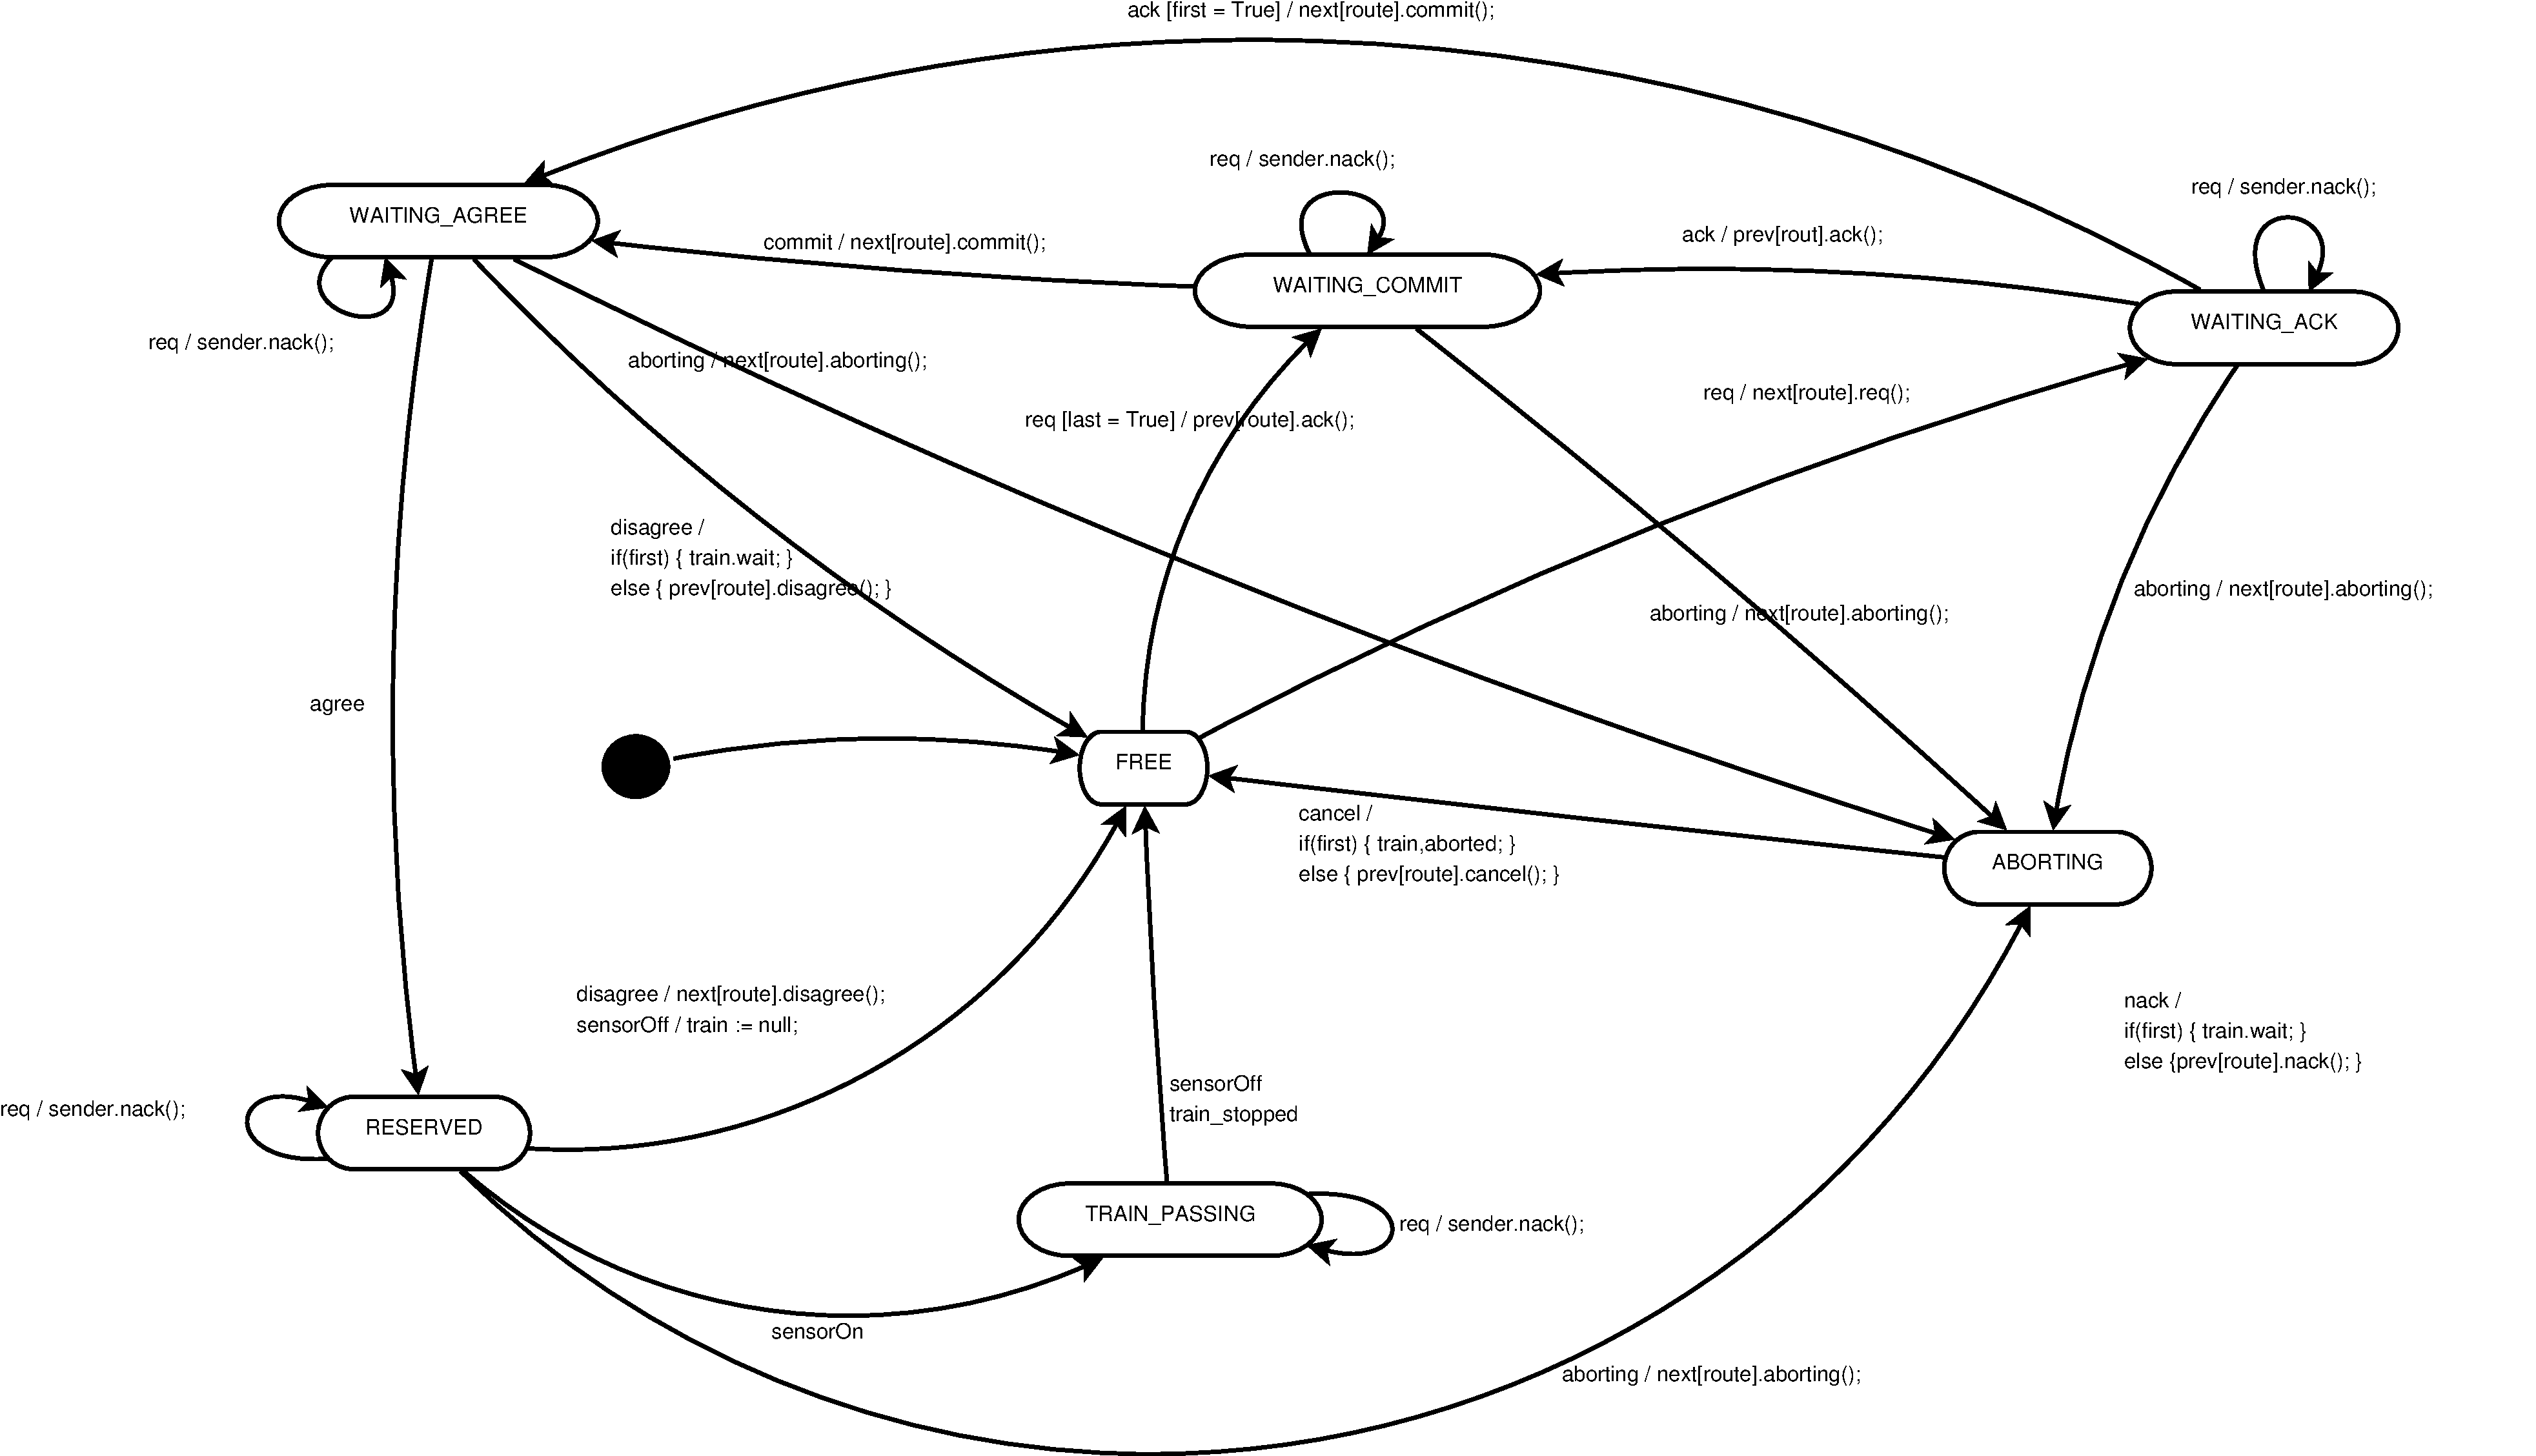
\includegraphics[width=24cm]{imgs/TrackCircuit.pdf}

\caption{Diagramma di variazione degli stati dello Scambio}\label{fig:Scambio}

\end{sidewaysfigure}

L’algoritmo di prenotazione implementato da questa classe è lo stesso di quello
della classe \textit{TrackCircuit} con alcune varianti dovute al fatto che:
\begin{enumerate}
  \item uno Scambio non può mai essere il primo o l’ultimo nodo di un itinerario,
quindi i messaggi possono essere solo ricevuti e spediti a Circuiti di Binario o
altri Scambi, mai a treni, di conseguenza non sono presenti salti in avanti da
\textit{FREE} a \textit{WAITING\_COMMIT} e da \textit{WAITING\_COMMIT} a
\textit{RESERVED}, o da \textit{WAITING\_ACK} a \textit{WAITING\_AGREE} propri
dei Circuiti di Binario iniziali e finali;
\item i treni non possono fermarsi su uno Scambio, quindi la richiesta di
 cancellazione di un itinerario non può avvenire su uno Scambio;
\item gli Scambi devono posizionarsi prima di permettere il passaggio del treno
(il posizionamento può fallire, ed è in questo caso che viene spedito un messaggio
di \textit{disagree}). 
\end{enumerate}

Ogni oggetto della classe \textit{Switch} ha due variabili aggiuntive rispetto
ai Circuiti di Binario, ossia \textit{reversed} e \textit{conf} che
rappresentano, rispettivamente, il posizionamento corrente (normale o rovescio)
e quale deve essere il posizionmento corretto per ogni itinerario. Per
permettere il posizionamento sono stati implementati due stati aggiuntivi,
\textit{CHECK\_POSITION e POSITIONING}, il loro ruolo è il seguente:
\begin{itemize}
  \item \textbf{CHECK\_POSITION}: lo Scambio si sposta in questo stato subito
  dopo aver ricevuto un agree e controlla se il suo posizionamento è corretto
  per l’itinerario richiesto (ossia se reversed == conf[route]). Se il
  posizionamento è giusto inoltra il messaggio \textit{agree} e si porta in
  \textbf{RESERVED} in attesa del transito del treno, se il posizionamento
  invece non è corretto allora passa allo stato \textit{POSITIONING};
  \item \textbf{POSITIONING}: in questo stato si aggiusta il posizionamento dello
	Scambio. Tale operazione può fallire, ossia non deterministicamente invece che
	passare allo stato \textit{RESERVED} inoltrando l’\textit{agree}, passa allo
	stato \textit{FREE} spedendo in entrambe le direzioni un \textit{disagree} che
	viene propagato su tutto l’itinerario cancellando, di fatto, la prenotazione.
\end{itemize}

\section{Modello del treno}
Il treno è stato implementato nella classe \textit{Train} rappresentata in
figura \ref{fig:Treno}.
\begin{sidewaysfigure}

\centering
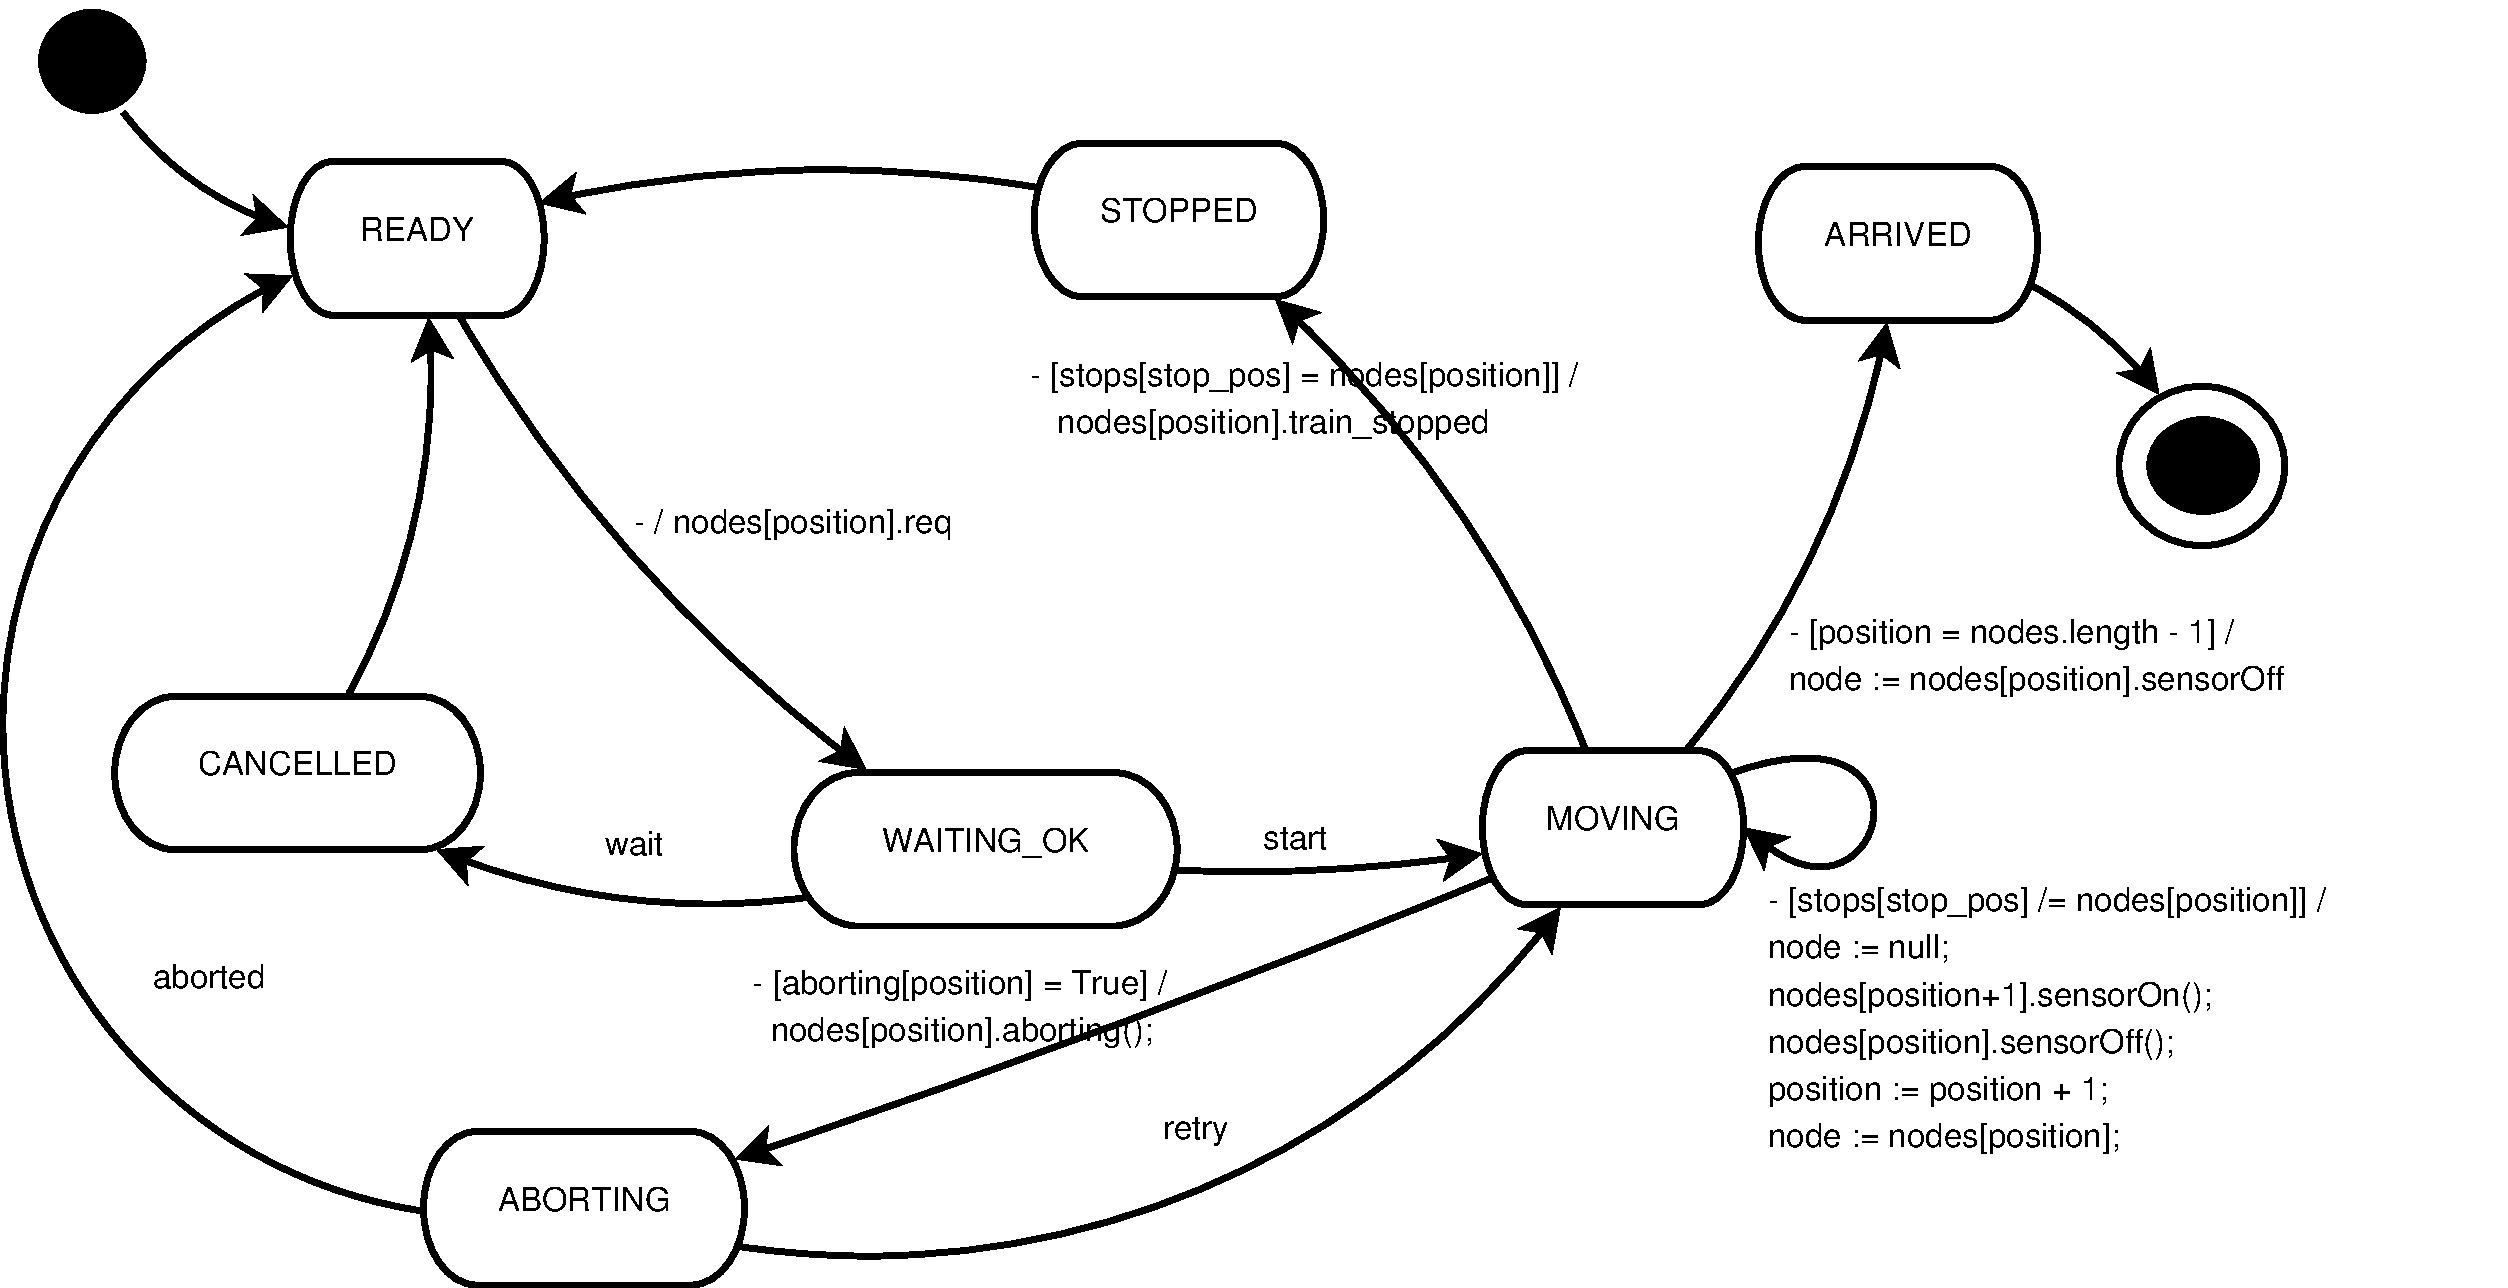
\includegraphics[width=24cm]{imgs/Train.pdf}

\caption{Diagramma di variazione degli stati del Treno}\label{fig:Treno}

\end{sidewaysfigure}

Il suo compito è quello di richiedere un itinerario inviando al Circuito di
Binario sul quale si trova un messaggio di \textit{req}. Se la prenotazione ha
successo, e quindi riceve in risposta un messaggio di \textit{start}, si muove
di nodo in nodo fino a raggiungere l’ultima stazione. A questo punto può
chiedere un nuovo itinerario oppure uscire dal tracciato, qual’ora si sia
fermato su un nodo esterno (ossia un Circuito di Binario in cui la variabile
\textit{outer\_station} == True).
In fase di istanziazione, ad ogni oggetto della classe \textit{Train} sono
assegnati:
\begin{itemize}
  \item un vettore di interi routes, rappresentante gli itinerari che il treno
  deve percorrere prima di fermarsi; 
  \item un vettore (nodes) contenente i nodi che compongono tutti gli
  itinerari da percorrere (tale vettore viene utilizzato durante la fase di
  movimento per sapere qual è il successivo nodo verso cui muoversi);
  \item un vettore di stazioni (stops) che indica su quali Circuiti di Binario
  il treno deve fermarsi;
  \item un vettore di nodi (aborting) che contiene i nodi sui quali il treno
  simula un malfunzionamente e invia la richiesta di cancellazione dell’itinerario.
\end{itemize}
Nella fase iniziale, il treno cicla fra gli stati \textit{READY} ed
\textit{WAITING\_OK} fino a quando non riceve una conferma positiva (messaggio
start) alla richiesta di prenotazione del primo itinerario. Se la prenotazione
non è andata a buon fine, ossia un nodo risulta già prenotato da un altro treno,
il messaggio di ritorno sarà un \textit{wait} e quindi il treno si riporta nello
stato \textit{CANCELLED} e, successivamente, nello stato \textit{READY} in attesa di tentare una nuova prenotazione.
Durante il movimento il treno si sposta da un nodo al successivo inviando messaggi
di sensorOn al nodo su cui entra e sensorOff al nodo dal quale esce. La chiamata
a \textit{sensorOff} di fatto riporta il nodo di uscita nello stato
\textit{FREE} rendendolo disponibile per una nuova prenotazione.
Quando il treno giunge alla fine di un itinerario segnalerà la fermata al
Circuito di Binario sul quale si trova per mezzo di un messaggio
\textit{train\_stopped} e torna nello stato \textit{READY} pronto per inviare la
richiesta di prenotazione per l’itinerario successivo.Se siamo giunti alla fine
dell’ultimo itinerario e la stazione è un nodo esterno il messaggio 
di \textit{sensorOff} permetterà anche l’uscita del treno dall’intero tracciato.

\section{Modello del Semaforo}
Il semaforo viene modellato con la classe \textit{Semaphore} rappresentata il cui diagramma di stato è in figura \ref{fig:semaforo}.
\begin{sidewaysfigure}

\centering
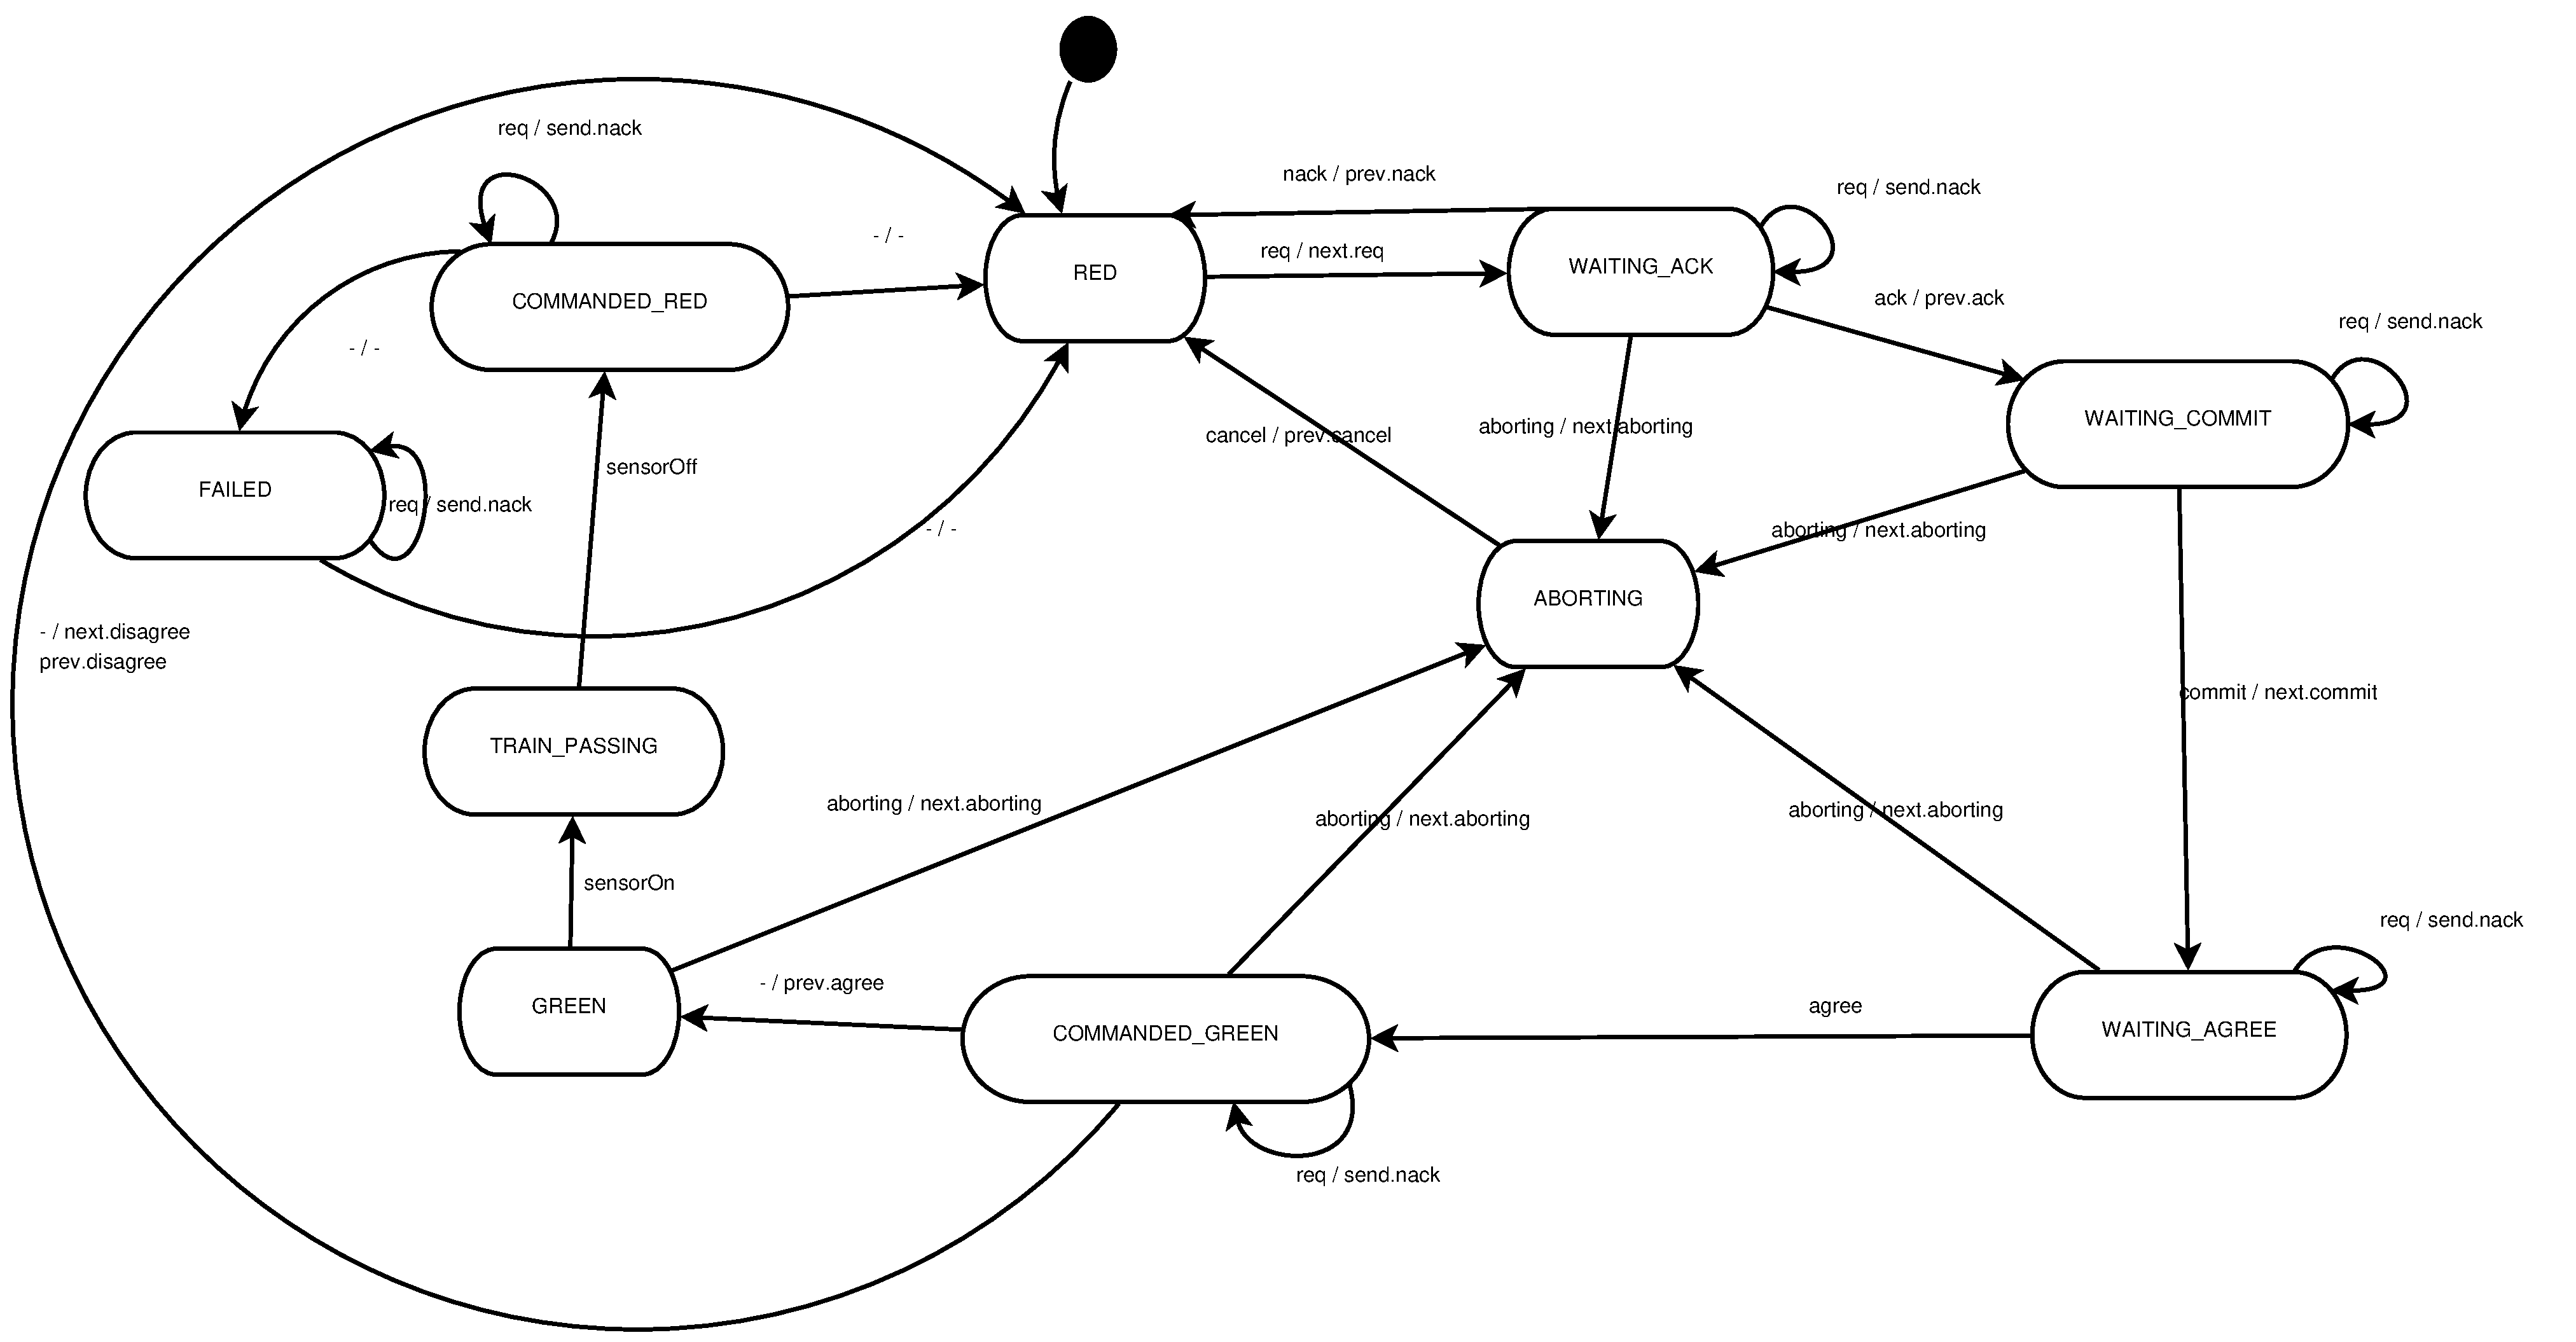
\includegraphics[width=24cm]{imgs/Semaphore.eps}

\caption{Diagramma di variazione degli stati del Semaforo}\label{fig:semaforo}

\end{sidewaysfigure}

Il semaforo, per la semantica della rete, non può essere il termine di un
itinerario, quindi ha all'interno dell'algoritmo di prenotazione solo
responsabilità di ricezione e inoltro dei segnali in arrivo e variazione del
proprio stato. La commutazione del segnale proposto è soggetta a fallimenti.

I segnali elaborati dal \textit{Semaphore} sono:
\begin{itemize}
  \item \textbf{Request} Il segnale \textit{req} dà inizio alla procedura per la prenotazione del nodo. Viene accettato
  e inoltrato al nodo successivo se lo stato del semaforo è \textit{RED}
  commutandolo in \textit{WAITING\_ACK}. La ricezione della
  \textit{request} in qualsiasi altro stato genera una risposta negativa attraverso il segnale
  \textit{nack}.
  \item \textbf{Acknowledgement} Il segnale \textit{ack} indica un riscontro posivito della richiesta di prenotazione da
  parte dei successivi nodi dell'itinerario. Il compito del semaforo è
  propagare il segnale e porre il suo stato in \textit{WAITING\_COMMIT}.
  \item \textbf{Negative Acknowledgement} Rappresentato dal
  segnale\textit{nack} indica un rifiuto della richiesta di prenotazione da parte dei successivi nodi
  dell'itinerario. Il semaforo propaga il \textit{nack} verso il \textit{Circuito di Binario} dove
  risiede il treno richiedente e ritorna nel suo stato iniziale \textit{RED}.
  \item \textbf{Commit} Il segnale \textit{commit} rappresenta il comando di conferma prenotazione inviata dal treno. Il
  semaforo propaga il segnale e si pone nello stato \textit{WAITING\_AGREE}
  \item \textbf{Agree} Il segnale \textit{agree} rappresenta il segnale finale della procura \emph{2PC}. Il semaforo che
  riceve questo segnale prima di inoltrarlo al nodo precedente dell'itinerario
  cambia il suo stato in \textit{COMMANDED\_GREEN}.
  \item \textbf{Abort} \textit{aborting} è il segnale per comunicare ai nodi dell'itinerario il
  fallimento del treno. I nodi, ed in particolare il semaforo, si pongono nello stato
  \textit{ABORTING}.
  \item \textbf{Cancel} \textit{cancel} è il segnale di conferma della ricezione di \textit{aborting} da parte dell'itinerario successivo al semaforo.
  Nel caso del semaforo comporta il passaggio di stato a \textit{RED}.
\end{itemize}

Gli stati possibili della classe \textit{Semaphore} sono:
\begin{itemize}
  \item \textbf{RED} Lo stato di attesa per la prenotazione.
  \item \textbf{WAITING\_ACK} ha ricevuto la richiesta ed è in attesa di
  \textit{ack}.
  \item \textbf{WAITING\_COMMIT} ha ricevuto l'\textit{ack} e lo ha inoltrato,
  quindi è in attesa di un \textit{commit}. 
  \item \textbf{WAITING\_AGREE} ha ricevuto il \textit{commit} e lo ha
  inoltrato, quindi è in attesa di un \textit{agree}. 
  \item \textbf{TRAIN\_PASSING} un treno si trova sul semaforo.
  \item \textbf{ABORTING} il semaforo ha ricevuto un messaggio di
  \textit{aborting} ed è in attesa di ricevere il \textit{cancel}
  \item \textbf{COMMANDED\_RED} stato in cui viene simulato la variazione del colore del semaforo in rosso. 
  La commutazione di colore può non deterministicamente fallire; quindi può passare allo stato \textit{FAILED} o \textit{RED}. Il fallimento comporta la mancata liberazione del nodo rendendo impossibile nuove prenotazioni.
  \item \textbf{COMMANDED\_GREEN} stato in cui viene simulato la variazione del colore del semaforo in verde. 
  La commutazione di colore può non deterministicamente fallire; può passare allo stato \textit{RED} se fallisce o \textit{GREEN} se la commutazione ha successo. Il fallimento comporta la mancata prenotazione dell'itinerario.
  \item \textbf{GREEN} stato di prenotazione effettuata con successo e di
  riservazione del semaforo per l'itinerario.
  \item \textbf{FAILED} stato del semaforo nel caso di fallimento di
  commutazione di colore da \textit{COMMANDED\_RED}. Esiste la possibilità di riparazione che riporta da questo stato in \textit{RED}.  La commutazione senza la ricezione di segnali evidenzia quindi la temporaneità del fallimento del semaforo.
   
\end{itemize}

%\chapter{Modellazione del sistema}

%come l'interlocking è stato implementato: scelte implementative
% nostro apporto al modello

\chapter{Safety e Stabilizzazione}
\label{cap:properties}
%Descrizione delle proprietà da garantire
Il sistema di interlocking distribuito da noi realizzato soddisfa la proprietà della \emph{stabilizzazione}.

La proprietà di \emph{stabilizzazione} può essere così enunciata:

\textit{per ogni richiesta di itinerario compiuta da un treno, posto al punto di inizio dell'itinerario, esiste una computazione che porta il treno al punto di fine dell'itinerario, e tutte le computazioni alternative (per effetto di guasti o altri motivi) producono un \emph{abort della richiesta}}.

In \emph{Computation Tree Logic (CTL)} questa proprietà viene descritta come:
\begin{lstlisting}
AG (locomotive_request implies AF (locomotive_arrived or locomotive_cancelled))
\end{lstlisting}

In particolare:
\begin{itemize}
\item \verb!locomotive_request! rappresenta la condizione di richiesta di itinerario di un treno;
\item \verb!locomotive_arrived! rappresenta la condizione di arrivo del treno al punto di fine itinerario;
\item \verb!locomotive_cancelled! rappresenta la condizione di \emph{abort della richiesta di itinerario}.
\end{itemize}

Tutte le condizioni specificate sono state implementate mediante il meccanismo delle astrazioni sugli stati, fornito dallo strumento di modellazione \emph{UMC}.

Il modello sviluppato, oltre a garantire la \emph{stabilizzazione}, soddisfa anche la importante proprietà della \emph{Safety}. Tale proprietà viene soddisfatta quando non vi sono incidenti tra i treni, ovvero essi non si trovano contemporaneamente nello stesso circuito di binario.

La formula in \emph{CTL} per testare tale proprietà è:
\begin{lstlisting}
AG ( not crash )
\end{lstlisting}
ove condizione di crash viene determinata dalla contemporanea presenza dei due treni sullo stesso nodo.
 
\chapter{Simulazione}
\label{cap:simulation}
% casi di test trattati
\section{Verifica della stabilizzazione}
La simulazione del modello è stata eseguita tramite una richiesta di itinerario da parte di un treno. 

Come si può notare in figura \ref{lst:itinerario}, in questa richiesta vengono esercitati tutti i possibili 15 itinerari, opportunamente concatenati di modo tale che l'ultimo nodo di ciascun itinerario intermedio coincida con il primo nodo dell'itinerario successivo.

Il test effettuato mostra che, su questa complessa configurazione, la proprietà di \emph{stabilizzazione} viene soddisfatta.

\begin{lstlisting}[numbers=left,
numberstyle=\tiny,caption={Simulazione di itinerario effettuata},
label=lst:itinerario]
GA1 A W1 GA2 N1 W2 GA4
GA4 F W2 GA2 P1 W1 GA1
GA1 A W1 GA3 N2 W3 W2 GA4
GA4 F W2 W3 GA3 P2 W1 GA1
GA1 A W1 GA2
GA2 P1 W1 GA1
GA1 A W1 GA3
GA3 P2 W1 GA1
GA1 A W1 GA3 N2 W3 GA5
GA5 S10 W3 GA3
GA3 N2 W3 W2 GA4
GA4 F W2 GA2
GA2 N1 W2 GA4
GA4 F W2 W3 GA3
GA3 N2 W3 GA5
\end{lstlisting}

\section{Verifica della safety}
Si è poi testato il modello rispetto alla proprietà di \emph{Safety}. A tal fine, si è istanziato due treni concorrenti con itinerari incidenti. La simulazione e la successiva verifica della formula di safety \verb!AG (not crash )! hanno portato a esito positivo. Le rotte sottoposte ai due treni sono state:

\begin{lstlisting}[numbers=left,
numberstyle=\tiny,caption={Simulazione di itinerario del primo treno},
label=lst:itinerario2]
GA4 F W2 W3 GA3 P2 W1 GA1
\end{lstlisting}
\begin{lstlisting}[numbers=left,
numberstyle=\tiny,caption={Simulazione di itinerario del secondo treno},
label=lst:itinerario3]
GA1 A W1 GA3 N2 W3 GA5
\end{lstlisting}


\chapter{Conclusioni}
\label{cap:conclusions}
In conclusione il modello da noi sviluppato riesce a permettere la prenotazione di un itinerario da parte di uno o più treni e gestire il sistema di segnalazione (i semafori) in maniera coerente in ottemperanza con la proprietà di \emph{stabilizzazione}. Inoltre viene garantita l'assenza di incidenti tra più treni preservando la \emph{safety} del sistema. 

I possibili itinerari sono stati esaustivamente testati concatenandoli tra loro e usando un apposito script per la generazione automatica delle configurazione da sottoporre al model checker. Sia in \cite{Paolieri} che in \cite{RossettoRocciolo} si lamentava la mancanza di un tale tool per rendere agevole la fase di test e stesura di configurazione di una eventuale rete ferroviaria diversa.

\appendix

\chapter{UML Model Checker}
\section{pippo}
%copia spudorata


\label{cap:code}
\begin{lstlisting}[caption={modello della classe Train}]
Class Train is

  Signals:
    start, wait, aborted, retry;

  Vars:
    routes: int[];
    route_pos: int := 0;
    nodes: obj[];
    position: int := 0;
    stops: obj[];
    stop_pos: int := 0;
    node: obj;
    aborting: bool[];

  State Top = READY, WAITING_OK, MOVING, ARRIVED, STOPPED, ABORTING, CANCELLED

  Transitions:
    READY -> WAITING_OK { - / 
    nodes[position].req(self, nodes[position], routes[route_pos]); }

    WAITING_OK -> CANCELLED { wait }  
    WAITING_OK -> MOVING { start }
    WAITING_OK -> ABORTING { - [aborting[position] = True] / 
    nodes[position].aborting(self, nodes[position], routes[route_pos]); }
    
    CANCELLED -> READY

    MOVING -> ABORTING { - [aborting[position] = True 
    and position < nodes.length - 1 and stops[stop_pos] /= nodes[position]] / 
    nodes[position].aborting(self, nodes[position], routes[route_pos]); }
    
    MOVING -> MOVING { - [aborting[position] = False 
    and position < nodes.length - 1 
    and stops[stop_pos] /= nodes[position]] /                    
                   node := null; --perche' queste azioni non sono atomiche!
                   -- sempre perche' non sono operazioni atomiche
                   -- il treno si trova per un istante su due nodi cosi da
                   -- evitare una doppia prenotazione. Quindi si setta prima 
                   -- su ON il nuovo
                   -- nodo e poi su OFF il nodo che viene lasciato.
    nodes[position + 1].sensorOn(self, nodes[position + 1], routes[route_pos]);
    nodes[position].sensorOff(self, nodes[position], routes[route_pos]);
    position := position + 1;
    node := nodes[position];
    }

    MOVING -> STOPPED { - [stops[stop_pos] = nodes[position] 
    and position < nodes.length - 1] 
    / nodes[position].train_stopped(self); }
    MOVING -> ARRIVED  { - [position = nodes.length - 1] 
    / node := null; 
    node := nodes[position].sensorOff(self, nodes[position], routes[route_pos]); }
    
    STOPPED -> READY { - [position < nodes.length - 1] /
                   stop_pos := stop_pos + 1;
                   route_pos := route_pos + 1;
    }
    
    ABORTING -> READY { aborted / 
    aborting[position] := False; }
    ABORTING -> MOVING { retry / 
    aborting[position] := False; aborting[position + 1] := True; }

end Train
\end{lstlisting}
\begin{lstlisting}[caption={modello della classe TrackCircuit}]
Class TrackCircuit is

  Signals:
    req(sender: obj, dest: obj, route: int);        
    ack(sender: obj, dest: obj, route: int);
    nack(sender: obj, dest: obj, route: int);
    commit(sender: obj, dest: obj, route: int);
    agree(sender: obj, dest: obj, route: int);
    disagree(sender: obj, dest: obj, route: int);
    train_stopped(sender: obj);
    aborting(sender: obj, dest: obj, route: int);
    cancel(sender: obj, dest: obj, route: int);

  Operations:
    sensorOn(sender: obj, dest: obj, route: int);
    sensorOff(sender: obj, dest: obj, route: int);

  Vars:
    next: obj[];
    prev: obj[];
    train: obj := null;
    outer_station: bool;

  State Top = FREE, WAITING_ACK, WAITING_COMMIT, WAITING_AGREE, RESERVED, 
  TRAIN_PASSING, ABORTING

  Transitions:
    FREE -> WAITING_ACK { req(sender, dest, route) [(train=null or sender=train) 
    and next[route] /= null] /
     next[route].req(self, next[route], route); }
    FREE -> WAITING_COMMIT { req(sender, dest, route) [(train=null or sender=train) 
    and next[route] = null] / 
    prev[route].ack(self, prev[route], route); }
    FREE -> FREE { req(sender, dest, route) [train/=null and sender/=train] 
    / sender.nack(self, sender, route); }

    WAITING_ACK -> WAITING_COMMIT { ack(sender, dest, route) 
    [prev[route] /= null and train = null] / 
    prev[route].ack(self, prev[route], route); }
    WAITING_ACK -> WAITING_AGREE{ ack(sender, dest, route) [train /= null] / 
    next[route].commit(self, next[route], route); }
    WAITING_ACK -> FREE { nack(sender, dest, route_id) 
    [(prev[route] = null) 
    and (train /= null)] / 
    train.wait; }
    WAITING_ACK -> FREE { nack(sender, dest, route_id) 
    [prev[route] /= null] / 
    prev[route].nack(self, prev[route], route); }
    WAITING_ACK -> WAITING_ACK { req(sender, dest, route) / 
    sender.nack(self, sender, route); }
    WAITING_ACK -> ABORTING { aborting(sender, dest, route) / 
    next[route].aborting(self, next[route], route); }

    WAITING_COMMIT -> WAITING_AGREE{ commit(sender, dest, route) 
    [next[route] /= null] /  next[route].commit(self, next[route], route); }
    WAITING_COMMIT -> Top.RESERVED{ commit(sender, dest, route) 
    [next[route] = null] / 
    prev[route].agree(self, prev[route], route); }
    WAITING_COMMIT -> WAITING_COMMIT { req(sender, dest, route) / 
    sender.nack(self, sender, route); }
    WAITING_COMMIT -> ABORTING { aborting(sender, dest, route) 
    [next[route] /= null] / 
    next[route].aborting(self, next[route], route); }
    WAITING_COMMIT -> FREE { aborting(sender, dest, route) 
    [next[route] = null] / 
    prev[route].cancel(self, prev[route], route); }

    WAITING_AGREE -> Top.RESERVED { agree(sender, dest, route) [prev[route] /= null 
    and train = null] / prev[route].agree(self, prev[route], route); }
    WAITING_AGREE -> Top.RESERVED { agree(sender, dest, route) [train /= null] / 
    train.start; }
    WAITING_AGREE -> FREE { disagree(sender, dest, route_id) 
    [(prev[route] = null) and (train /= null)] / 
    train.wait; }
    WAITING_AGREE -> FREE { disagree(sender, dest, route_id) 
    [prev[route] /= null] / 
    prev[route].disagree(self, prev[route], route); }
    WAITING_AGREE -> WAITING_AGREE { req(sender, dest, route) / 
    sender.nack(self, sender, route); }
    WAITING_AGREE -> ABORTING { aborting(sender, dest, route) / 
    next[route].aborting(self, next[route], route); }

    Top.RESERVED -> TRAIN_PASSING { sensorOn(sender,dest,route) / 
    train := sender; }
    Top.RESERVED -> FREE { disagree(sender, dest, route) / 
    if next[route] /= null then 
    { next[route].disagree(self, next[route], route) }; }
    Top.RESERVED -> FREE { sensorOff(sender,dest,route) / 
    train := null; }
    Top.RESERVED -> Top.RESERVED { req(sender, dest, route) / 
    sender.nack(self, sender, route); }
    Top.RESERVED -> ABORTING { aborting(sender, dest, route) 
    [next[route] /= null] / 
    next[route].aborting(self, next[route], route); }
    Top.RESERVED -> FREE { aborting(sender, dest, route) 
    [next[route] = null] / 
    prev[route].cancel(self, prev[route], route); }

    TRAIN_PASSING -> FREE { sensorOff(sender,dest,route) 
    [next[route] = null] / 
    if(outer_station = True) { train := null; return null;} 
    else { return self; } }
    TRAIN_PASSING -> FREE { sensorOff(sender,dest,route) 
    [next[route] /= null] / 
    train := null; }
    TRAIN_PASSING -> FREE { train_stopped(sender) 
    [train = sender] }
    TRAIN_PASSING -> TRAIN_PASSING { req(sender, dest, route) / 
    sender.nack(self, sender, route); }
    TRAIN_PASSING -> ABORTING { aborting(sender, dest, route) / 
    next[route].aborting(self, next[route], route); }

    ABORTING -> FREE { cancel(sender, dest, route) 
    [train /= null] / 
    train.aborted; }
    ABORTING -> FREE { cancel(sender, dest, route) 
    [train = null and prev[route] /= null] / 
    prev[route].cancel(self, prev[route], route); }

end TrackCircuit

\end{lstlisting}
\begin{lstlisting}[caption={modello della classe Switch}]
Class Switch is

  Signals:
    req(sender: obj, dest: obj, route: int);        
    ack(sender: obj, dest: obj, route: int);
    nack(sender: obj, dest: obj, route: int);
    commit(sender: obj, dest: obj, route: int);
    agree(sender: obj, dest: obj, route: int);
    disagree(sender: obj, dest: obj, route: int);
    aborting(sender: obj, dest: obj, route: int);
    cancel(sender: obj, dest: obj, route: int);

  Operations:
    sensorOn(sender: obj, dest: obj, route: int);  
    sensorOff(sender: obj, dest: obj, route: int);

  Vars:
    next: obj[];             
    prev: obj[];             
    conf: bool[];
    reversed: bool := False; 
    train: obj := null;      
    requested_route: int;         

  State Top = FREE, WAITING_ACK, WAITING_COMMIT, 
  WAITING_AGREE, POSITIONING, RESERVED, 
  TRAIN_PASSING, CHECK_POSITION, ABORTING
  
  State WAITING_ACK Defers req(sender: obj, dest: obj, route: int)

  Transitions:
    FREE -> WAITING_ACK { req(sender, dest, route) / 
    next[route].req(self, next[route], route); }

    WAITING_ACK -> WAITING_COMMIT { ack(sender, dest, route) / 
    prev[route].ack(self, prev[route], route); }
    WAITING_ACK -> FREE { nack(sender, dest, route) / 
    prev[route].nack(self, prev[route], route); }
    WAITING_ACK -> WAITING_ACK { req(sender, dest, route) / 
    sender.nack(self, sender, route); }
    WAITING_ACK -> ABORTING { aborting(sender, dest, route) / 
    next[route].aborting(self, next[route], route); }

    WAITING_COMMIT -> WAITING_AGREE { commit(sender, dest, route) / 
    				next[route].commit(self, next[route], route); }
    WAITING_COMMIT -> WAITING_COMMIT { req(sender, dest, route) / 
    sender.nack(self, sender, route); }
    WAITING_COMMIT -> ABORTING { aborting(sender, dest, route) / 
    next[route].aborting(self, next[route], route); }

    WAITING_AGREE -> FREE { disagree(sender, dest, route) / 
    prev[route].disagree(self, prev[route], route); }
    WAITING_AGREE -> WAITING_AGREE { req(sender, dest, route) / 
    sender.nack(self, sender, route); }
    WAITING_AGREE -> CHECK_POSITION { agree(sender, dest, route) / 
    requested_route := route; }
    WAITING_AGREE -> ABORTING { aborting(sender, dest, route) / 
    next[route].aborting(self, next[route], route); }

    CHECK_POSITION -> Top.RESERVED { - [reversed = conf[requested_route]] / 
    prev[requested_route].agree(self, prev[requested_route], 
    requested_route); }
    CHECK_POSITION -> POSITIONING { - [reversed /= conf[requested_route]] }
    CHECK_POSITION -> CHECK_POSITION { req(sender, dest, route) / 
    sender.nack(self, sender, route); }
    CHECK_POSITION -> ABORTING { aborting(sender, dest, route) / 
    next[route].aborting(self, next[route], route); }

    POSITIONING -> Top.RESERVED { - / reversed := not reversed; 
    prev[requested_route].agree(self, prev[requested_route], 
    requested_route); }
    POSITIONING -> FREE  { - / 
    prev[requested_route].disagree(self, prev[requested_route], 
    requested_route); 
    next[requested_route].disagree(self, next[requested_route], 
    requested_route); }
    POSITIONING -> POSITIONING { req(sender, dest, route) / 
    sender.nack(self, sender, route); }
    POSITIONING -> ABORTING { aborting(sender, dest, route) / 
    next[route].aborting(self, next[route], route); }

    Top.RESERVED -> TRAIN_PASSING { sensorOn(sender,dest,route) / 
    train := sender; }
    Top.RESERVED -> FREE { disagree(sender, dest, route) / 
    next[route].disagree(self, next[route], route); }
    Top.RESERVED -> Top.RESERVED { req(sender, dest, route) / 
    sender.nack(self, sender, route); }
    Top.RESERVED -> ABORTING { aborting(sender, dest, route) / 
    next[route].aborting(self, next[route], route); }

    TRAIN_PASSING -> FREE { sensorOff(sender,dest,route) / 
    train := null; }
    TRAIN_PASSING -> TRAIN_PASSING { req(sender, dest, route) / 
    sender.nack(self, sender, route); }
    TRAIN_PASSING -> TRAIN_PASSING { aborting(sender, dest, route) 
    [train /= null and sender = train] / train.retry; }

    ABORTING -> FREE { cancel(sender, dest, route) / 
    prev[route].cancel(self, prev[route], route); }

end Switch
\end{lsrlisting}

\begilsstlisting}[caption={modello della classe Semaphore}]
Class Semaphore is

  Signals:
    req(sender: obj, dest: obj, route: int);        
    ack(sender: obj, dest: obj, route: int);
    nack(sender: obj, dest: obj, route: int);
    commit(sender: obj, dest: obj, route: int);
    agree(sender: obj, dest: obj, route: int);
    disagree(sender: obj, dest: obj, route: int);
    aborting(sender: obj, dest: obj, route: int);
    cancel(sender: obj, dest: obj, route: int);

  Operations:
    sensorOn(sender: obj, dest: obj, route: int);  
    sensorOff(sender: obj, dest: obj, route: int);

  Vars:
    next: obj[];             
    prev: obj[];             
    train: obj := null;      
    requested_route: int;
    color_red: bool := True ;          

  State Top = RED, WAITING_ACK, WAITING_COMMIT, WAITING_AGREE, 
  COMMANDED_RED, COMMANDED_GREEN, TRAIN_PASSING, GREEN, ABORTING, FAILED
  
  State WAITING_ACK Defers req(sender: obj, dest: obj, route: int)

  Transitions:
    RED -> WAITING_ACK { req(sender, dest, route) / 
    next[route].req(self, next[route], route); }

    WAITING_ACK -> WAITING_COMMIT { ack(sender, dest, route) / 
    prev[route].ack(self, prev[route], route); }
    WAITING_ACK -> RED { nack(sender, dest, route) / 
    prev[route].nack(self, prev[route], route); }
    WAITING_ACK -> WAITING_ACK { req(sender, dest, route) / 
    sender.nack(self, sender, route); }
    WAITING_ACK -> ABORTING { aborting(sender, dest, route) / 
    next[route].aborting(self, next[route], route); }

    WAITING_COMMIT -> WAITING_AGREE { commit(sender, dest, route) / 
    next[route].commit(self, next[route], route); }
    WAITING_COMMIT -> WAITING_COMMIT { req(sender, dest, route) / 
    sender.nack(self, sender, route); }
    WAITING_COMMIT -> ABORTING { aborting(sender, dest, route) / 
    next[route].aborting(self, next[route], route); }

    WAITING_AGREE -> RED { disagree(sender, dest, route) / 
    prev[route].disagree(self, prev[route], route); }
    WAITING_AGREE -> WAITING_AGREE { req(sender, dest, route) / 
    sender.nack(self, sender, route); }
    WAITING_AGREE -> COMMANDED_GREEN { agree(sender, dest, route) / 
    requested_route := route; }
    WAITING_AGREE -> ABORTING { aborting(sender, dest, route) / 
    next[route].aborting(self, next[route], route); }

    COMMANDED_GREEN -> Top.GREEN { - / 
    prev[requested_route].agree(self, 
    prev[requested_route], requested_route); 
    color_red := False; }
    COMMANDED_GREEN -> RED  { - / 
    prev[requested_route].disagree(self, 
    prev[requested_route], requested_route); 
    next[requested_route].disagree(self, 
    next[requested_route], requested_route); }
    
    COMMANDED_GREEN -> COMMANDED_GREEN { req(sender, dest, route) / 
    sender.nack(self, sender, route); }
    
    COMMANDED_GREEN -> ABORTING { aborting(sender, dest, route) / 
    next[route].aborting(self, next[route], route); }

    Top.GREEN -> TRAIN_PASSING { sensorOn(sender,dest,route) / 
    train := sender; }
    Top.GREEN -> Top.GREEN { req(sender, dest, route) / 
    sender.nack(self, sender, route); }
    Top.GREEN -> ABORTING { aborting(sender, dest, route) / 
    next[route].aborting(self, next[route], route); }

    TRAIN_PASSING -> COMMANDED_RED { sensorOff(sender,dest,route) / 
    train := null; }
    TRAIN_PASSING -> TRAIN_PASSING { req(sender, dest, route) / 
    sender.nack(self, sender, route); }
    TRAIN_PASSING -> TRAIN_PASSING { aborting(sender, dest, route) 
    [train /= null and sender = train] / train.retry; }
 
    COMMANDED_RED -> COMMANDED_RED { req(sender, dest, route) / 
    sender.nack(self, sender, route); }
    COMMANDED_RED -> FAILED
    COMMANDED_RED -> RED {- / 
    color_red := True;}
    
    FAILED -> FAILED { req(sender, dest, route) / 
    sender.nack(self, sender, route); }
    FAILED -> RED {- / 
    color_red := True;}

    ABORTING -> RED { cancel(sender, dest, route) / 
    prev[route].cancel(self, prev[route], route); }

end Semaphore
\end{lstlisting}

\begin{lstlisting}[caption={oggetti istanziati nella simulazione}]
Objects

GA1: TrackCircuit (
 train => null, 
    outer_station => True,
 prev => [null,null,null,null,null,null,W1,null,W1,null,W1,null,W1
 ,null,null],
 next => [A,A,A,A,A,null,null,null,null,null,null,null,null,null,
 null]);
A: Semaphore (
    train => null,
 prev => [GA1,GA1,GA1,GA1,GA1,null,null,null,null,null,null,null,
 null,null,null],
 next => [W1,W1,W1,W1,W1,null,null,null,null,null,null,null,null,
 null,null]);
W1: Switch (
 conf => [False, False, False, False, False, False, False, False, 
 False, False, False, False, False, True, True],
    train => null,
 prev => [A,A,A,A,A,null,P1,null,P2,null,P1,null,
 P2,null,null],
 next => [GA2,GA2,GA3,GA3,GA3,null,GA1,null,GA1,null,
 GA1,null,GA1,null,null]);
GA2: TrackCircuit (
 train => null, 
    outer_station => False,
 prev => [W1,W1,null,null,null,W2,W2,null,null,null,null,null,
 null,null,null],
 next => [null,N1,null,null,null,null,P1,null,null,null,P1,N1,
 null,null,null]);
N1: Semaphore (
    train => null,
 prev => [null,GA2,null,null,null,null,null,null,null,null,null,
 GA2,null,null,null],
 next => [null,W2,null,null,null,null,null,null,null,null,null,
 W2,null,null,null]);
W2: Switch (
 conf => [False, False, False, False, False, False, False, False, 
 False, False, False, 
 False, False, True, True],
 prev => [null,N1,null,W3,null,F,F,F,F,null,null,N1,null,W3,null],
 next => [null,GA4,null,GA4,null,GA2,GA2,W3,W3,null,null,GA4,null,
 GA4,null]);
GA4: TrackCircuit (
 train => null, 
    outer_station => True,
 prev => [null,W2,null,W2,null,null,null,null,null,null,null,W2,
 null,W2,null],
 next => [null,null,null,null,null,F,F,F,F,null,null,null,null,
 null,null]);
GA3: TrackCircuit (
 train => locomotive, 
    outer_station => False,
 prev => [null,null,W1,W1,W1,null,null,W3,W3,W3,null,null,null,
 null,null],
 next => [null,null,null,N2,N2,null,null,null,P2,null,null,null,
 P2,N2,N2]);
N2: Semaphore (
    train => null,
 prev => [null,null,null,GA3,GA3,null,null,null,null,null,null,
 null,null,GA3,GA3],
 next => [null,null,null,W3,W3,null,null,null,null,null,null,
 null,null,W3,W3]);
W3: Switch (
 conf => [False, False, False, False, False, False, False, 
 False, False, False, False, 
 False, False, True, True],
 prev => [null,null,null,N2,N2,null,null,W2,W2,S10,null,
 snull,null,N2,N2],
 next => [null,null,null,W2,GA5,null,null,GA3,GA3,GA3,null,
 null,null,W2,GA5]);
GA5: TrackCircuit (
 train => null, 
    outer_station => False,
 prev => [null,null,null,null,W3,null,null,null,null,null,null,null,
 null,null,W3],
 next => [null,null,null,null,null,null,null,null,null,S10,null,null,
 null,null,null]);
F: Semaphore (
    train => null,
 prev => [null,null,null,null,null,GA4,GA4,GA4,GA4,null,null,null,null,
 null,null],
 next => [null,null,null,null,null,W2,W2,W2,W2,null,null,null,null,null,null]);
P1: Semaphore (
    train => null,
 prev => [null,null,null,null,null,null,GA2,null,null,null,GA2,null,null,
 null,null],
 next => [null,null,null,null,null,null,W1,null,null,null,W1,null,null,null,null]);
P2: Semaphore (
    train => null,
 prev => [null,null,null,null,null,null,null,null,GA3,null,null,null,GA3,
 null,null],
 next => [null,null,null,null,null,null,null,null,W1,null,null,null,W1,
 null,null]);
S10: Semaphore (
    train => null,
 prev => [null,null,null,null,null,null,null,null,null,GA5,null,null,null,
 null,null],
 next => [null,null,null,null,null,null,null,null,null,W3,null,null,null,
 null,null]);
 
 locomotive: Train (
 	routes => [ 1,6,3,8,0,10,2,12,4,9,13,5,11,7,14],
 	nodes => [ GA1,A,W1,GA2,N1,W2,GA4,F,W2,GA2,P1,W1,GA1,A,W1,GA3,N2,W3,W2,
 	GA4,F,W2,W3,
 	GA3,P2,W1,GA1,A,W1,GA2,P1,W1,GA1,A,W1,GA3,P2,W1,GA1,A,W1,GA3,N2,W3,GA5,
 	S10,W3,GA3,
 	N2,W3,W2,GA4,F,W2,GA2,
 	N1,W2,GA4,F,W2,W3,GA3,N2,W3,GA5],
 	aborting => [False,False,False,False,False,False,False,False,False,False,
 	False,False,False,False,False,False,False,False,False,False,False,False,
 	False,False,False,False,False,False,False,False,False,False,False,False,
 	False,False,False,False,False,False,False,False,False,False,False,False,
 	False,False,False,False,False,False,False,False,
 	False,False,False,False,False,False,False,False,
 	False,False,False],
 	stops => [GA4,GA1,GA4,GA1,GA2,GA1,GA3,GA1,GA5,GA3,GA4,GA2,
 	GA4,GA3,GA5],
 	node => GA1
 );
 
\end{lstlisting}

\begin{lstlisting}[caption={Astrazioni per la verifica delle proprieta'}]
Abstractions {
  Action $1($*) -> $1($*)
    
  State inState(locomotive.ARRIVED) -> locomotive_arrived

  State inState(locomotive.CANCELLED) -> locomotive_cancelled

  State inState(locomotive.WAITING_OK) -> locomotive_request
  }
\end{lstlisting}

\bibliography{bibliography}
\end{document}


